\documentclass[10pt]{beamer}
%% beamer template and options 
\mode<presentation>
{
  \usetheme{CambridgeUS}
  \usefonttheme{serif}
  \useoutertheme{default}
}\setbeamertemplate{navigation symbols}{} 



\usepackage[utf8]{inputenc}
\usepackage{xcolor,comment,cancel,tabularx,multirow}
\specialcomment{extended}{}{}    
\excludecomment{extended}
\usepackage{../styles/authordate1-4-beamer}

\usepackage{pgfplots}
\usepackage{xspace}
\usepackage{amsmath}
\usepackage{wasysym}
\usepackage{tikz}
\usetikzlibrary{automata,fit}
\usetikzlibrary{arrows}
\usetikzlibrary{shapes}
\usetikzlibrary{snakes}
\usetikzlibrary{arrows.meta,intersections}
\tikzstyle{every picture}+=[remember picture]
\usetikzlibrary{decorations.markings}





\title[IDL@BME-BIN] % (optional, use only with long paper titles)
{Introduction to Deep Learning} 
\subtitle{2D Convolution for image }

\author[A. Allauzen] % (optional, use only with lots of authors)
{Alexandre Allauzen}



\institute[ESPCI/Dauphine/PSL] % (optional, but mostly needed)
{

\includegraphics[height=3em]{../logos/espci_blue.png}\hfill
\raisebox{1.75ex}{
\includegraphics[height=1.5em]{../logos/dauphine.png}}\\
\hfill
\includegraphics[height=3em]{../logos/logomiles_white.pdf}
}




\date{12 and 13/10/20} % (optional)





\DeclareMathOperator*{\argmax}{argmax}
\DeclareMathOperator*{\argmin}{argmin}

\newcommand{\ngram}{\mbox{$n$-gram}\xspace} 



%% important : red + bf 
\def\important#1{{\bf \color{red} #1\/}}


%%% basics : 
\newcommand{\real}{\ensuremath{\mathbb{R}}}
\newcommand{\vct}[1]{\ensuremath{\mathbf{#1}}} % a vector / matrix is in bold
\newcommand{\seq}[1]{\ensuremath{\boldsymbol{#1}}}

\newcommand{\transp}[1]{\ensuremath{{#1}^{t} }} % transposition 
%\newcommand{\scal}[2]{\left\langle #1 , #2 \right\rangle} % scalair
%product
\newcommand{\scal}[2]{#1^t#2} % scalair product
\newcommand{\mydot}[2]{\ensuremath{ \transp{#1} #2}} % dot prod
\newcommand{\norm}[1]{\ensuremath{|| #1 ||}} % l2
\newcommand{\normabs}[1]{\ensuremath{ || #1 ||_{1} }} % l1




% vertical vector 
\newcommand{\vv}[1]{
	\left(
	\begin{array}[c]{c}
		#1 
	\end{array}
	\right)
}
% backeted vertical vector 
\newcommand{\vvb}[1]{
	\left[
	\begin{array}[c]{c}
		#1 
	\end{array}
	\right]
}
% raw vertical vector 
\newcommand{\vvr}[1]{
	\begin{array}[c]{c}
		#1 
	\end{array}
}





% words sequences sentences 
\newcommand{\ws}{{w}} % 
\newcommand{\wseq}{{\mathbf{\ws}}} % 
\newcommand{\length}{{L}} % 
\newcommand{\wsseq}[2]{{\ws_{#1}^{#2}}} % word subsequence
\newcommand{\word}[1]{{\it #1}} % an example
\newcommand{\vocab}{{\mathcal{V}}} % vocab

\newcommand{\asymb}{\ensuremath{a}} % symbol of *one* element of the
                                % alignment sequence
\newcommand{\ssymb}{\ensuremath{s}} % symbol of *one* element of the source
\newcommand{\tsymb}{\ensuremath{t}} % symbol of *one* element of the target


\newcommand{\aseq}{\ensuremath{\mathbf{\asymb}}} % alignment sentence
\newcommand{\sseq}{\ensuremath{\mathbf{\ssymb}}} % source sentence
\newcommand{\tseq}{\ensuremath{\mathbf{\tsymb}}} % target sentence


% misc 
\newcommand{\BigO}[1]{\ensuremath{\operatorname{O}\bigl(#1\bigr)}}
\newcommand{\bos}{\texttt{\textless s\textgreater}} 
\newcommand{\eos}{\texttt{\textless/s\textgreater}} 


% machine learning i/o and parameters ...
% params for model 
\newcommand{\param}{\ensuremath{\theta}} 
\newcommand{\params}{\ensuremath{\boldsymbol{\theta}}}
\newcommand{\nfeats}{\ensuremath{D}} % 

\newcommand{\x}{\ensuremath{\seq{x}}} % 
\newcommand{\X}{\ensuremath{\seq{X}}} % 
\newcommand{\y}{\ensuremath{\seq{y}}} % 
\newcommand{\z}{\ensuremath{\seq{z}}} % 
\newcommand{\w}{\ensuremath{\seq{w}}} % 
\newcommand{\pa}{\ensuremath{\seq{a}}} % 
\newcommand{\pb}{\ensuremath{\seq{b}}} % 

\newcommand{\W}{\seq{W}}
\newcommand{\V}{\seq{V}}
\newcommand{\pgrad}[1]{\nabla_{#1}}
\newcommand{\vgrad}[2]{\ensuremath{\nabla_{#1} #2}}

%%%%%%% data and loss
\newcommand{\nsamples}{\ensuremath{N}}
\newcommand{\ploss}{\ensuremath{l}} % for one datapoint
\newcommand{\class}{\ensuremath{{c}}} %
\newcommand{\rvclass}{\ensuremath{{C}}} %  the class as a RV 
\newcommand{\sid}[1]{\ensuremath{_{(#1)}}} % sample id
\newcommand{\tid}[1]{_{(#1)}} % time index for parameters
\newcommand{\exi}{\ensuremath{\x\sid{i}}} % 
\newcommand{\classi}{\ensuremath{\class\sid{i}}} % 
\newcommand{\nclasses}{\ensuremath{C}} % 
\newcommand{\yi}{y\sid{i}}  % prediction for sample i 

\newcommand{\dataset}{\ensuremath{\mathcal{D}}} % training data
\newcommand{\datax}{\ensuremath{\mathcal{X}}} % training data, x part
\newcommand{\datay}{\ensuremath{\tilde{\mathcal{Y}}}} % training data y part  
\newcommand{\datac}{\ensuremath{\tilde{\mathcal{C}}}} % training data c part (classes)
\newcommand{\ty}{\ensuremath{\tilde{y}}} % the supervised answer
\newcommand{\fullloss}{\ensuremath{\mathcal{L}(\params;\dataset)}}

%%% 
\newcommand{\nlaw}{\mathcal{N}}
\newcommand{\bern}{\ensuremath{\pi}}



%%%%%%%%%%%%%%%%%%%%%%%%%%%%%%%%%%%%%%%%%%%%%%%%%%%%%%%%%%%%
% a vector as a grid 
% 1: x 
% 2: y
% 3: the number of cells 
% The template :
% \node[rectangle,rounded corners,  draw, fill=red!20, text width=0.3*\textwidth, minimum height=6ex]  (label) at (0,0) {Hello} ;
\newcommand{\xvector}[3]{%
  \draw[step=.25] (#1-0.001,#2) grid (#1+0.25,#2+#3*0.25 );%
}

% notations 
% a layer l 
% input x^{(l)}
% output y^{(l)}
%  y^{(l)} = f^{(l)}( W^{(l)} input)
% note that 
% y_i = W_i,: x
% W_ij : x_j -> y_i  
% k is for the class
% l for the layer 


%%%%%%% to define layers math notations 
\newcommand{\inp}{\ensuremath{\x}}
\newcommand{\outp}{\ensuremath{\seq{y}}}
\newcommand{\lid}[1]{\ensuremath{^{(#1)}}}

%%%%%%% data and loss
\newcommand{\dlta}{\ensuremath{\delta}} % gradient component of pre-activation
\newcommand{\vdlta}{\ensuremath{\seq{\delta}}} % gradient vector of pre-activation

\colorlet{darkgreen}{green!50!black}


%% draw one layer 
\newcommand{\layer}{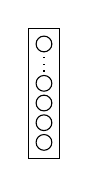
\begin{tikzpicture}[baseline=0.5ex]%
    \foreach \y in {0.25,0.5,...,1}{ 
      \draw (0,\y) circle  (0.1);%
    }
    \draw[dotted] (0.0, 1.15) -- (0.0,1.35); 
    \draw (0,1.5) circle (0.1);
    \draw (-0.2,0.05) rectangle (0.2,1.7);
\end{tikzpicture}}

%% draw connection
\newcommand{\connection}{\begin{tikzpicture}[baseline=0.5ex]%
    \draw[->] (0,0.85) -- (1.0,0.85);
\end{tikzpicture}}
%% dotted connection
\newcommand{\dotted}{\begin{tikzpicture}[baseline=0.5ex]%
    \draw[dotted,thick] (0,0.85) -- (0.5,0.85);%
\end{tikzpicture}}

\newcommand{\raiseW}{2ex}
% for computational graph
\newcommand{\vnode}{\node}
\newcommand{\funnode}{\node[minimum size=1.5,rectangle,draw=green,fill=green!20]}
\newcommand{\inlinefnode}[1]{\raisebox{-5pt}{\tikz{\funnode {#1}}}}



\newcommand{\justunder}{0.5cm}
\newcommand{\largeurUn}{0.8}
\newcommand{\largeurDeux}{0.7}
\setbeamercolor{postit}{fg=black,bg=red!30}
\setbeamercolor{mygreen}{fg=black,bg=green!20}
\setbeamercolor{myred}{fg=black,bg=red!20}
\setbeamercolor{darkpostit}{fg=black,bg=red!64}
\setbeamercolor{text}{fg=black,bg=red!10}


%%%%%%%%%% NNet for NLP
%% draw one layer  
\newcommand{\wemb}{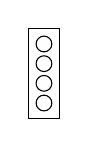
\begin{tikzpicture}[baseline=0.5ex]%
    \foreach \y in {0.25,0.5,...,1}{ 
      \draw (0,\y) circle  (0.1);%
    }
    \draw (-0.2,0.05) rectangle (0.2,1.2);
\end{tikzpicture}}

\newcommand{\worddim}{\ensuremath{K}} % dimension of the word embeddings
\newcommand{\wvector}{\ensuremath{\vct{v}}} % word vector
\newcommand{\wmatrix}{\ensuremath{\vct{R}}} % word matrix
\newcommand{\dvector}{\ensuremath{\vct{d}}} % document vector



%%%%%%%%% macro et redefinition 
\AtBeginSection[]
{
  \begin{frame}<beamer>
    \frametitle{Outline}
    \tableofcontents[currentsection]
  \end{frame}
}


\begin{document}
\tikzset{->-/.style={decoration={
  markings,
  mark=at position .5 with {\arrow{>}}},postaction={decorate}}}

\begin{frame}
  \titlepage
\end{frame}

\begin{frame}<beamer>
  \frametitle{Outline}
  \tableofcontents
\end{frame}
 






%%%%%%%%%%%%%%%%%%%%%%%%%%%%%%%%%%%%%%%%%%%%%%%%%%%%%%%%%%%%%%%%%%%%%%
\section{Introduction and reminder}
%%% reminder: sequence of discrete symbols
% + exemples of Human activity / audio classification
% embeddings
% COnv 1D
% Pooling
%%% Exo: conv1D and padding
%%% Exo: Pooling derivative 
%%% links : 
% https://arxiv.org/pdf/1607.02383.pdf for music classif
% and https://arxiv.org/pdf/1904.08990.pdf
% for heart signal : https://asp-eurasipjournals.springeropen.com/articles/10.1186/s13634-019-0651-3
% MFCC and 1D conv + DAE
%%%%%%%%%%%%%%%%%%%%%%%%%%%%%%%%%%%%%%%%%%%%%%%%%%%%%%%%%%%%%%%%
% This intro/reminder comes after a first course on sequence
% processing with 1D NNet for discrete sequence. 
% reminder: sequence of discrete symbols
% - examples of application
% - + exemples of Human activity / audio classification
% - embeddings
% - COnv 1D
% - Pooling

% Alphabet = set of nucleotides: 
% A,C,G,T
\newcommand{\cga}{{\color{red!70!black} A}}
\newcommand{\cgc}{{\color{blue!70!black} C}}
\newcommand{\cgg}{{\color{yellow!70!black} G}}
\newcommand{\cgt}{{\color{green!70!black} T}}

\begin{frame}{Sequence of discrete symbols classification }
  \begin{block}{Movie review classification}
    \begin{center}
      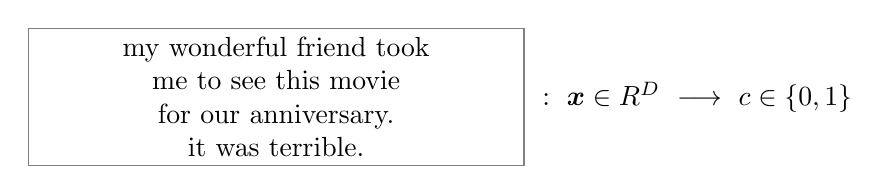
\begin{tikzpicture}
        %%%%%%%%%%%%%%%%%%%%% 
        \node[anchor=east,draw=gray,text width=0.5\textwidth,align=center] (review) at
        (0,0) {my wonderful friend took me to see this movie \\for our
          anniversary. \\ it was terrible.};
        %%%%%%%%%%%%%%%%%%%%% 
        \node[anchor=west] (txt) at (0.1,0) {$: \ \x \in \real^{\nfeats} \ \longrightarrow \ \class \in\{0, 1\}$};
      \end{tikzpicture}
    \end{center}
  \end{block}
  \begin{block}{Enhancer Identification in  DNA Sequences}
    \begin{center}
      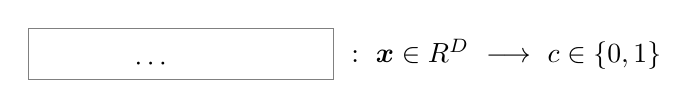
\begin{tikzpicture}
        %%%%%%%%%%%%%%%%%%%%% 
        \node[anchor=east,draw=gray,text width=0.3\textwidth,align=center] (review) at
        (0,0) {\cga~\cgt~\cgc~\cgg~\cga~\cgt~\cgc~\cgg\\$\cdots$~\cgg~\cgt~\cga~\cga~\cgt~\cgc~\cgg};
        %%%%%%%%%%%%%%%%%%%%% 
        \node[anchor=west] (txt) at (0.1,0) {$: \ \x \in \real^{\nfeats} \ \longrightarrow \ \class \in\{0, 1\}$};
      \end{tikzpicture}
    \end{center}
  \end{block}
  \begin{itemize}
  \item $\dataset= (\exi , \classi )_{i=1}^{\nsamples}$ 
  \item The input is a sequence $\rightarrow$ how to build $\x$ ? 
  \item A sequence of discrete symbols $\in \vocab$
  \item Symbols  interact with each other, the neighborhood is important
  \end{itemize}
\end{frame}


%%%%%%%%%%%%%%%%%%%%%%%%%%%%%%%%%%%%%%%%%%%%%%%%%%%%%%%%%%%%%%%%%%
\begin{frame}{Embedding of discrete symbols}
    \begin{center}
      \begin{displaymath}
          \begin{array}{lcccccccc}
            \seq{s}=&[ &\cgc&\cga&\cgt&\cgt&\cgg&\cgt
                        &]\\
            &&\downarrow &\downarrow &\downarrow &\downarrow &\downarrow &\downarrow \\
            \textrm{Look-up}&&\wemb &\wemb &\wemb &\wemb &\wemb &\wemb  \\
               &&\wvector_{\cgc}&\wvector_{\cga}&\wvector_{\cgt}&\wvector_{\cgt}&\wvector_{\cgg}&\wvector_{\cgt} \\
          \end{array}
        \end{displaymath}
        {\huge $\downarrow$} \\
        \tikz{\draw[step=0.5,black,thin] (0,0) grid (3,2);}
    \end{center}
\end{frame}

%%%%%%%%%%%%%%%%%%%%%%%%%%%%%%%%%%%%%%%%%%%%%%%%%%%%%%%%%%%%%%%%%%
% In pytorch the indices are :
% batch, channel, data-point
% The data point for a 1D input is (t,d)
% For an image it is (x,y)
\begin{frame}{Convolution 1D}
  \framesubtitle{Extract a frame, or a window, and apply a ``filter''}
  \begin{columns}
    \column{0.6\textwidth}
    %%% the input : a matrix + window
    \begin{center}
    The input sequence of  $L=6$ \\vectors in $\real^{\nfeats}$,  $\nfeats=4$ \\[1ex]
    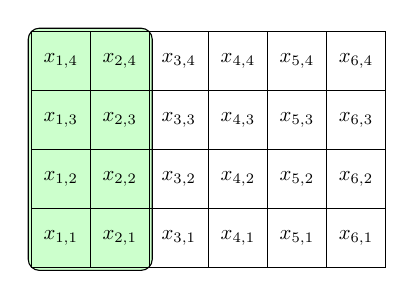
\begin{tikzpicture}[scale=0.75,every node/.style={scale=0.75}]
      % the window
      % offset for x and y of .5 + a bit more 
      \draw[fill=green!20,rounded corners] (0.45,0.45) rectangle (2.55,4.55); % green 
      %% the grid 
      \foreach \l in {1,2,...,4}
      \foreach \c in {1,2,...,6}
      {
        \draw (\c,\l) +(-.5,-.5) rectangle ++(.5,.5);
        \draw (\c,\l) node{$x_{\c,\l}$};
      }
    \end{tikzpicture}
  \end{center}
    \column{0.6\textwidth}
    \begin{center}
    The filter:\\kernel size of $ks=2$\\[1ex]
    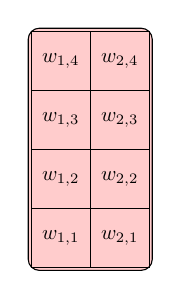
\begin{tikzpicture}[scale=0.75,every node/.style={scale=0.75}]
      % the window
      % offset for x and y of .5 + a bit more 
      \draw[fill=red!20,rounded corners] (0.45,0.45) rectangle (2.55,4.55); % green 
      
      %% the grid 
      \foreach \l in {1,2,...,4}
      \foreach \c in {1,2}
      {
        \draw (\c,\l) +(-.5,-.5) rectangle ++(.5,.5);
        \draw (\c,\l) node{$w_{\c,\l}$};
      }
    \end{tikzpicture}
  \end{center}
\end{columns}
\begin{block}{The output value (output channel)}
  $$
  \textrm{At time }t = 1,\ {\color{red!70!black} h_1} = \sum_{i,j} {\color{red!70!black}w_{i,j}}\times  {\color{green!70!black}x_{i,j}}
  $$
\end{block}
\end{frame}



%%%%%%%%%%%%%%%%%%%%%%%%%%%%%%%%%%%%%%%%%%%%%%%%%%%%%%%%%%%%%%%%%%%%%%%%%%%%%%%%%%%%%%%% 
\begin{frame}{Convolution 1D}
  \framesubtitle{With 2 output channels}
  \begin{columns}
    \column{0.6\textwidth}
    %%% the input : a matrix + window
    \begin{center}
      $L=6$,  $\nfeats=4$ \\[1ex]
      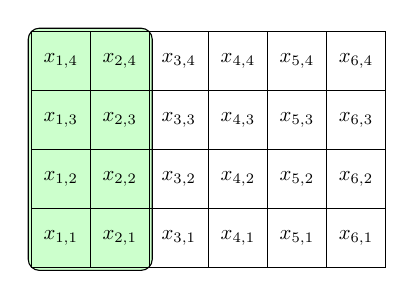
\begin{tikzpicture}[scale=0.75,every node/.style={scale=0.75}]
        % the window
        % offset for x and y of .5 + a bit more 
        \draw[fill=green!20,rounded corners] (0.45,0.45) rectangle (2.55,4.55); % green 
        %% the grid 
        \foreach \l in {1,2,...,4}
        \foreach \c in {1,2,...,6}
        {
          \draw (\c,\l) +(-.5,-.5) rectangle ++(.5,.5);
          \draw (\c,\l) node{$x_{\c,\l}$};
        }
      \end{tikzpicture}
    \end{center}
    \column{0.4\textwidth}
    \begin{center}
      Filters:kernel size of $ks=2$\\[1ex]
      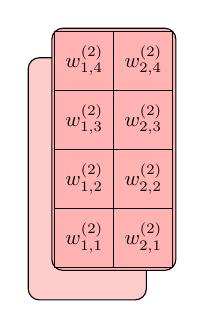
\begin{tikzpicture}[scale=0.75,every node/.style={scale=0.75}]
        % the window
        % offset for x and y of .5 + a bit more 
        \draw[fill=red!20,rounded corners] (0.05,-0.05) rectangle (2.05,4.05); % first 
        \draw[fill=red!30,rounded corners] (0.45,0.45) rectangle (2.55,4.55); 
        %% the grid 
        \foreach \l in {1,2,...,4}
        \foreach \c in {1,2}
        {
          \draw (\c,\l) +(-.5,-.5) rectangle ++(.5,.5);
          \draw (\c,\l) node{$w_{\c,\l}\lid{2}$};
        }
      \end{tikzpicture}
    \end{center}
  \end{columns}
  \begin{block}{The output value (output channel)}
    \begin{align*}
      {\color{red!70!black} h_{1,1}} &= \sum_{i,j} {\color{red!70!black}w_{i,j}\lid{1}}\times  {\color{green!70!black}x_{i,j}} \\
      {\color{red!70!black} h_{2,1}} &= \sum_{i,j} {\color{red!70!black}w_{i,j}\lid{2}}\times  {\color{green!70!black}x_{i,j}} 
    \end{align*}
  \end{block}
\end{frame}




%%%%%%%%%%%%%%%%%%%%%%%%%%%%%%%%%%%%%%%%%%%%%%%%%%%%%%%%%%%%%%%%%%
\begin{frame}{Audio classification / segmentation}
  \framesubtitle{\cite{Jang19Music}}
  \begin{center}
    \includegraphics[width=0.6\textwidth]{../figs/music_speech}    
  \end{center}
  \begin{itemize}
  \item Classification at each time step
  \item But the context is crucial (for the input and the output) ! 
  \item \important{Spectrogram ?}
  \end{itemize}
\end{frame}


%%%%%%%%%%%%%%%%%%%%%%%%%%%%%%%%%%%%%%%%%%%%%%%%%%%%%%%%%%%%%%%%%%
\begin{frame}{Interlude: the input spectrogram}
  \begin{center}
    \includegraphics[width=0.5\textwidth]{../figs/speech_1}\\
    $\downarrow$ \\
    Segmentation in frames (Hamming window)\\
    $\downarrow$ \\
    F.F.T \\
    $\downarrow$ \\
    Mel Filters \\
    $\downarrow$ \\
    Log\\
    $\downarrow$ \\
    D.C.T  \\
    $\downarrow$ \\
    \includegraphics[width=0.5\textwidth]{../figs/speech_2}\\
  \end{center}
\end{frame}



\begin{frame}{Human activity Recognition}
  \begin{block}{The data}
    10k samples of fixed length (128 points at 50kHz)
    \footnote{\url{https://archive.ics.uci.edu/ml/datasets/human+activity+recognition+using+smartphones}}:
    \begin{itemize}
    \item x, y, and z accelerometer data (linear acceleration) 
    \item and the three gyroscopic data (angular velocity)
    \end{itemize}
    The classes are: Walking, Upstairs,  Downstairs,  Sitting,  Standing, Laying. 
  \end{block}
  \begin{itemize}
  \item[$\rightarrow$] Two different input channels (accelerometer and
    gyroscopic).
  \item[$\rightarrow$] How to define a convolution filter for two
    input channels ?
  \item[$\rightarrow$] The sequence is long but of fixed size, the
    overall max-pooling is maybe not the best option.
  \end{itemize}
\end{frame}


\begin{frame}{Convolution 1D with 2 input channels}
    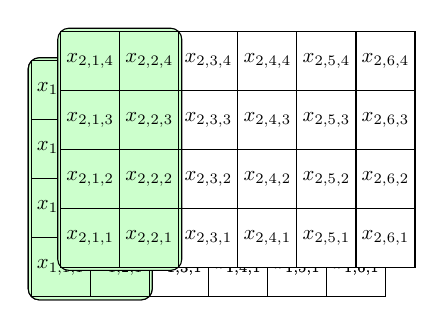
\begin{tikzpicture}[scale=0.75,every node/.style={scale=0.75}]
      % the window 
      % offset for x and y of .5 + a bit more
      %%%% channel 1 
      \draw[fill=green!20,rounded corners] (0.45,0.45) rectangle (2.55,4.55); % green 
      %% the grid 
      \foreach \l in {1,2,...,4}
      \foreach \c in {1,2,...,6}
      {
        \draw (\c,\l) +(-.5,-.5) rectangle ++(.5,.5);
        \draw (\c,\l) node{$x_{1,\c,\l}$};
      }
      %%%% channel 1 
      \draw[fill=green!20,rounded corners] (0.45,0.45) rectangle (2.55,4.55); % green 
      %% the grid 
      \foreach \l in {1,2,...,4}
      \foreach \c in {1,2,...,6}
      {
        \draw (\c,\l) +(-.5,-.5) rectangle ++(.5,.5);
        \draw (\c,\l) node{$x_{1,\c,\l}$};
      }
      %\pause
      %%%% channel 2 
      \draw[fill=white] (1,1) rectangle (7,5);
      \draw[fill=green!20,rounded corners] (0.95,0.95) rectangle (3.05,5.05); % green 
      %% the grid 
      \foreach \l in {1,2,...,4}
      \foreach \c in {1,2,...,6}
      {
        \draw (\c,\l) rectangle ++(1,1);
        \draw (\c,\l)+(0.5,0.5) node{$x_{2,\c,\l}$};
      }
    \end{tikzpicture}
    \hfill
    %\pause
    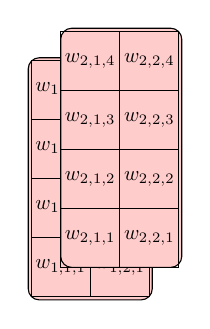
\begin{tikzpicture}[scale=0.75,every node/.style={scale=0.75}]
      %%% channel 1 
      % the window
      % offset for x and y of .5 + a bit more 
      \draw[fill=red!20,rounded corners] (0.45,0.45) rectangle (2.55,4.55); % green 
      %% the grid 
      \foreach \l in {1,2,...,4}
      \foreach \c in {1,2}
      {
        \draw (\c,\l) +(-.5,-.5) rectangle ++(.5,.5);
        \draw (\c,\l) node{$w_{1,\c,\l}$};
      }
      %\pause
      %%% channel 2
      \draw[fill=red!20,rounded corners] (1,1) rectangle (3.05,5.05); % green 
      %% the grid 
      \foreach \l in {1,2,...,4}
      \foreach \c in {1,2}
      {
        \draw (\c,\l) rectangle ++(1,1);
        \draw (\c,\l)+(0.5,0.5) node{$w_{2,\c,\l}$};
      }
    \end{tikzpicture}
    \begin{block}{The output value (output channel)}
      $$
      \textrm{At time }t = 1,\ {\color{red!70!black} h_1} = \sum_{k,i,j} {\color{red!70!black}w_{k,i,j}}\times  {\color{green!70!black}x_{k,i,j}}
      $$
    \end{block}
    We can have multiple input and output channels. 
  \end{frame}



  \begin{frame}{Convolution 1D and max-pooling in pytorch}
    \begin{columns}
      \column{0.5\textwidth}
      \begin{block}{Convolution 1D}
        torch.nn.Conv1d(
        \begin{itemize}
        \item in\_channels, 
        \item out\_channels, 
        \item kernel\_size, 
        \item stride=1, 
        \item padding=0,
        \item dilation=1, ...
        \end{itemize}
        )
      \end{block}
      \column{0.5\textwidth}
      \begin{block}{Max-Pooling 1D}
      torch.nn.MaxPool1d(
      \begin{itemize}
      \item kernel\_size, 
      \item stride=None, 
      \item padding=0, 
      \item dilation=1,
      \item return\_indices=False, 
      \item ceil\_mode=False
      \end{itemize}
      )
    \end{block}
    \end{columns}
  \end{frame}






%%%%%%%%%%%%%%%%%%%%%%%%%%%%%%%%%%%%%%%%%%%%%%%%%%%%%%%%%%%%%%%%%%%%%% 
\section{Convolution network for images}
%%%%%%%%%%%%%%%%%%%%%%%%%%%%%%%%%%%%%%%%%%%%%%%%%%%%%%%%%%%%%%%%%%%%%%%%%%%%%%%%%%%%%%%%
%% tikz draw a 3D representation of matrices for "image"
%% the tikz code 
%%%%%%%%%%%%%%%%%%%%%%%%%%%%%%%%%%%%%%%%%%%%%%%%%%%%%%%%%%%%%%%%%%%%%%%%%%%%%%%%%%%%%%%%
\newcommand{\tikzcube}[5]{% width, height, depth, color, scale 
    \foreach \x in {0,...,#1}
    {   \draw (\x*#5 ,0  ,#5*#3 ) -- (\x*#5 ,#5*#2 ,#5*#3 );
      \draw (\x*#5 ,#5*#2 ,#5*#3 ) -- (\x*#5 ,#5*#2 ,0  );
    }
    \foreach \x in {0,#2}
     {   \draw (#5*#1 ,\x*#5 ,#5*#3 ) -- (#5*#1 ,\x*#5 ,0  );
       \draw (0  ,\x*#5 ,#5*#3 ) -- (#5*#1 ,\x*#5 ,#5*#3 );
     }
     \foreach \x in {0,#3}
     {   \draw (#5*#1 ,0  ,\x*#5 ) -- (#5*#1 ,#5*#2 ,\x*#5 );
       \draw (0  ,#5*#2 ,\x*#5 ) -- (#5*#1 ,#5*#2 ,\x*#5 );
     }
    \draw[fill=#4!50,opacity=0.5] (0,0,#5*#3) rectangle (#5*#1,#5*#2,#5*#3);
    \draw[fill=#4!50] (#5*#1,0,0) -- (#5*#1,#5*#2,0) -- (#5*#1,#5*#2,#5*#3) -- (#5*#1,0,#5*#3) -- cycle ;
}

%%%%%%%%%%%%%%%%%%%%%%%%%%%%%%%%%%%%%%%%%%%%%%%%%%%%%%%%%%%%%%%%%%%%%%%%%%%%%%%%%%%%%%%%
%% The wrapper in a tikzpicture : scale can be 0.25 
%%%%%%%%%%%%%%%%%%%%%%%%%%%%%%%%%%%%%%%%%%%%%%%%%%%%%%%%%%%%%%%%%%%%%%%%%%%%%%%%%%%%%%%% 
\newcommand{\tikzcuboid}[5]{% width, height, depth, color, scale 
  \begin{tikzpicture}
    \tikzcube{#1}{#2}{#3}{#4}{#5}
  \end{tikzpicture}
}
%%%%%%%%%%%%%%%%%%%%%%%%%%%%%%%%%%%%%%%%%%%%%%%%%%%%%%%%%%%%%%%%%%%%%%%%%%%%%%%%%%%%%%%%
%% Shifted
%%%%%%%%%%%%%%%%%%%%%%%%%%%%%%%%%%%%%%%%%%%%%%%%%%%%%%%%%%%%%%%%%%%%%%%%%%%%%%%%%%%%%%%% 
\newcommand{\shiftedtikzcube}[7]{% width, height, depth, color, scale, xshift, yshift
    \foreach \x in {0,...,#1}
    {   \draw (\x*#5 +#6,0+#7  ,#5*#3 ) -- (\x*#5 +#6 ,#5*#2+#7 ,#5*#3 );
      \draw (\x*#5 +#6 ,#5*#2+#7 ,#5*#3 ) -- (\x*#5 +#6 ,#5*#2+#7 ,0  );
    }
    \foreach \x in {0,#2}
     {   \draw (#5*#1 +#6 ,\x*#5+#7 ,#5*#3 ) -- (#5*#1 +#6 ,\x*#5+#7 ,0  );
       \draw (0 +#6  ,\x*#5 +#7,#5*#3 ) -- (#5*#1 +#6 ,\x*#5+#7 ,#5*#3 );
     }
     \foreach \x in {0,#3}
     {   \draw (#5*#1+#6,0 +#7 ,\x*#5 ) -- (#5*#1 +#6 ,#5*#2 +#7,\x*#5 );
       \draw (0 +#6,#5*#2+#7 ,\x*#5 ) -- (#5*#1 +#6,#5*#2+#7 ,\x*#5 );
     }
    \draw[fill=#4!50,opacity=0.5] (0 +#6,0+#7,#5*#3) rectangle (#5*#1 +#6,#5*#2+#7,#5*#3);
    \draw[fill=#4!50] (#5*#1 +#6,0+#7,0) -- (#5*#1 +#6,#5*#2+#7,0) -- (#5*#1 +#6,#5*#2+#7,#5*#3) -- (#5*#1 +#6,0+#7,#5*#3) -- cycle ;
}



\begin{frame}{Image classification}
  \begin{center}
    An image = (2D array of values) $\times$ (number of channels)
  \end{center}
  \begin{block}{2D array}
    The spatial structure:
    \begin{itemize}
    \item A 2D real space
    \item With distance 
    \end{itemize}
  \end{block}
  \begin{block}{Channels}
    \begin{itemize}
    \item For image : R,G,B
    \item In fluid mechanics: pression, velocity, ... 
    \item In general: different measures on the same spatial domain
    \end{itemize}
  \end{block}
  \begin{block}{Sources}
    Many figures and examples are inspired by, or extracted from the
    course of the Stanford course of Fei-Fei Li.
    \begin{flushright}
      \small \url{http://cs231n.stanford.edu/}
    \end{flushright}
  \end{block}
\end{frame}

\begin{frame}{Image classification}
  \begin{center}
    \tikz[baseline=0]{ \node at (-2,0)
      {\includegraphics[height=0.25\textheight]{figs/mnist_5.pdf}}; %
      \node at (-0.4,0) {$\rightarrow$}; \xvector{0}{-0.75}{6} }
    $\x \in \real^{784} \ \longrightarrow \class  \in\{0, 1,2, \ldots ,9
    \}$
  \end{center}
  Another example with a color image (3 channels) of $32\times32$ pixels
  \begin{center}
    \tikz[baseline=0]{
      \shiftedtikzcube{3}{10}{10}{green}{0.25}{0}{-1}; 
      \node at (1,0) {$\rightarrow$}; \xvector{2}{-1.25}{10} }
    $\x \in \real^{3072} \ \longrightarrow \class  \in\{0, 1,2, \ldots ,9
    \}$
  \end{center}
\end{frame}


\begin{frame}{A simple 2D-convolution}
  \framesubtitle{One input channel and one output channel}
  \begin{itemize}
  \item Image of $(7,7)$
  \item Kernel size of $(3,3)$
  \item Stride of $(2,2)$ along line and column
\end{itemize}
  \begin{columns}
    \column{0.7\textwidth}
    \begin{center}
      \only<1>{Filter applied at $l=1$ and $c=1$\\[1ex]}
      \only<2>{Filter applied at $l=1$ and $c=3$\\[1ex]}
      \only<3>{Filter applied at $l=1$ and $c=5$\\[1ex]}
      \only<4>{Filter applied at $l=3$ and $c=1$\\[1ex]}
      \begin{tikzpicture}[scale=0.5,every node/.style={scale=0.75}]
        % the window
        % offset for x and y of .5 + a bit more/less 
        \only<1>{
          \draw[fill=green!20,rounded corners] (0.45,-0.45) rectangle (3.55,-3.55); % green
        }
        \only<2>{
          \draw[fill=green!20,rounded corners] (2.45,-0.45) rectangle (5.55,-3.55); % green
        }
        \only<3>{
          \draw[fill=green!20,rounded corners] (4.45,-0.45) rectangle (7.55,-3.55); % green
        }
        \only<4>{
          \draw[fill=green!20,rounded corners] (0.45,-2.45) rectangle (3.55,-5.55); % green
        }
        %% the grid 
        \foreach \l in {1,2,...,7}%{8,7,...,1}
        \foreach \c in {1,2,...,7}
        {
          \draw (\c,-\l) +(-.5,-.5) rectangle ++(.5,.5);
          \draw (\c,-\l) node{$x_{\l,\c}$};
        }
      \end{tikzpicture}
    \end{center}

    \column{0.3\textwidth}
    \begin{center}
      The filter or kernel is $3\times 3 $\\[1ex]
      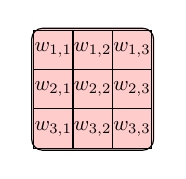
\begin{tikzpicture}[scale=0.5,every node/.style={scale=0.75}]
        % the window
        % offset for x and y of .5 + a bit more 
        \draw[fill=red!20,rounded corners] (0.45,-0.45) rectangle (3.55,-3.55); % green 
        
        %% the grid 
        \foreach \l in {1,2,3}
        \foreach \c in {1,2,3}
        {
          \draw (\c,-\l) +(-.5,-.5) rectangle ++(.5,.5);
          \draw (\c,-\l) node{$w_{\l,\c}$};
        }
      \end{tikzpicture}
    \end{center}
  \end{columns}
    $$
    \textrm{At position }l, \textrm{ and } c,\ {\color{red!70!black} h_{l,c}} = \sum_{i,j} {\color{red!70!black}w_{i,j}}\times  {\color{green!70!black}x_{l+i-1,c+j-1}}
  $$
\end{frame}

\begin{frame}{Convolution in 2D}
  \framesubtitle{The basics}
  \begin{columns}
    \column{0.6\textwidth}
    \begin{tabular}{lll}
      \begin{tabular}{c}
        \tikzcuboid{3}{10}{10}{green}{0.25}
      \end{tabular}
      & \begin{tabular}{c}
          $\longrightarrow$
        \end{tabular}
      & \begin{tabular}{c}
          \tikzcuboid{3}{3}{3}{red}{0.25}
        \end{tabular}
      \\
      $3\times 32\times 32$ image & &$3\times 5\times 5$ filter
    \end{tabular}
    \column{0.4\textwidth}
    Convolution of the filter  with the image:
    \begin{itemize}
    \item Sliding the filter along the two axis
    \item Computing the ``dot product'' at each step
    \item[$\rightarrow$] preserve the spatial structure along the channels
    \item[$\rightarrow$] each step extract a ``local'' and spatial feature
    \end{itemize}
  \end{columns}
\end{frame}

\begin{frame}{Convolution in 2D}
  \framesubtitle{With a single output channel}
  % \begin{center}
  %   \tikz[baseline=0]{
  %   \shiftedtikzcube{3}{10}{10}{green}{0.25}{0}{-1}; %% 
  %   \node at (1.5,0) {$\longrightarrow$}; 
  %   \shiftedtikzcube{3}{3}{3}{red}{0.25}{3}{0}; %%
  %   \node at (4.5,0) {$\longrightarrow$};
  %   \shiftedtikzcube{1}{8}{8}{red}{0.25}{6}{0}; %%
  % }
  % \end{center}


  \begin{center}
    \begin{tabular}{ccccc}
      \begin{tabular}{c}
        \tikzcuboid{3}{10}{10}{green}{0.25}
      \end{tabular}
      & \begin{tabular}{c}
          $\longrightarrow$
        \end{tabular}
      & \begin{tabular}{c}
          \tikzcuboid{3}{3}{3}{red}{0.25}
        \end{tabular}
      & \begin{tabular}{c}
          $\longrightarrow$
        \end{tabular}
      & \begin{tabular}{c}
          \tikzcuboid{1}{8}{8}{red}{0.25}
        \end{tabular}
      \\
      $3\times 32\times 32$ image & &$3\times 5\times 5$ filter & &$1 \times 28\times 28$ output 
    \end{tabular}
  \end{center}
\end{frame}

\begin{frame}{Convolution in 2D}
  \framesubtitle{Add a second output channel}
  % \begin{center}
  %   \tikz[baseline=0]{
  %   \shiftedtikzcube{3}{10}{10}{green}{0.25}{0}{-1}; %% 
  %   \node at (1.5,0) {$\longrightarrow$}; 
  %   \shiftedtikzcube{3}{3}{3}{red}{0.25}{3}{0}; %%
  %   \node at (4.5,0) {$\longrightarrow$};
  %   \shiftedtikzcube{1}{8}{8}{red}{0.25}{6}{0}; %%
  % }
  % \end{center}


  \begin{center}
    \begin{tabular}{ccccc}
      \begin{tabular}{c}
        \tikzcuboid{3}{10}{10}{green}{0.25}
      \end{tabular}
      & \begin{tabular}{c}
          $\longrightarrow$
        \end{tabular}
      & \begin{tabular}{c}
          \tikzcuboid{3}{3}{3}{red}{0.25}\\
          \tikzcuboid{3}{3}{3}{red}{0.25}\\
        \end{tabular}
      & \begin{tabular}{c}
          $\longrightarrow$
        \end{tabular}
      & \begin{tabular}{c}
          \tikzcuboid{2}{8}{8}{red}{0.25}
        \end{tabular}
      \\
      \begin{tabular}{c}
      $3\times 32\times 32$ \\image
      \end{tabular}
      &
      &\begin{tabular}{c}
         $2\times (3\times 5\times 5)$\\filters
       \end{tabular}
      &
      & \begin{tabular}{c}
          $2 \times 28\times 28$ \\ output
        \end{tabular}
    \end{tabular}
  \end{center}
\end{frame}


\begin{frame}{Motivation for convolution}
  \framesubtitle{Extract ``low level'' features}
  \begin{center}
    \only<1>{\includegraphics[width=0.8\textwidth]{../figs/image_and_filters_4}}
    \only<2>{\includegraphics[width=0.8\textwidth]{../figs/image_and_filters_1}}
    \only<3>{\includegraphics[width=0.8\textwidth]{../figs/image_and_filters_9}}
  \end{center}
\end{frame}


\begin{frame}{Max-pooling or Downsampling in 2D}
  \begin{block}{The goal}
    \begin{itemize}
    \item Convolution extracts local features (followed by non-linearity)
    \item Max-pooling acts as a selection, compression, or contraction operator
    \item The back-propagation promote feature saliency for each channel
    \end{itemize}
  \end{block}
  \begin{center}
    \includegraphics[width=0.7\textwidth]{../figs/pooling2D}
  \end{center}
\end{frame}

\begin{frame}{Architecture of deep convolution NNet for image processing}
  \framesubtitle{VGGNet~\cite{Simonyan15VGG}}
  \begin{center}
    \includegraphics[width=0.7\textwidth]{../figs/vgg16}
  \end{center}
  Conv. layers with kernel size of $3\times 3$, stride and padding,
  followed by pooling layers (max on $2\times 2$ with stride 2).
\end{frame}

\begin{frame}{Architecture of deep convolution NNet for image processing}
  \framesubtitle{A summary}
  \begin{block}{The basic block}
    \begin{itemize}
    \item A convolution layer with a ReLU activation followed by a max-pooling layer
    \item An alternative is two convolution layers in a Residual block (ResNet~\cite{He16Residual})
    \end{itemize}
  \end{block}
  \begin{center}
    \includegraphics[width=0.5\textwidth]{../figs/perf_imagenet.pdf}
  \end{center}
\end{frame}



\begin{frame}{Residual block }
  \begin{block}{Residual block}
    \begin{columns}
    \column{0.5\textwidth}
    From~\cite{He16Residual}
    \begin{itemize}
    \item Add a skip connection
    \item The model learn the "residual"
      $$
      \y = \mathcal{F}(\x) = \x + \mathcal{R}(\x)
      $$
    \end{itemize}
      \column{0.5\textwidth}
      \begin{center}
        \includegraphics[width=0.8\textwidth]{../figs/residual}
      \end{center}
    \end{columns}
    A simple version of highway networks~\cite{Srivastava15Highway}
  \end{block}
  \begin{block}{ResNet}
      \begin{center}
        \includegraphics[width=\textwidth]{../figs/resnet}
      \end{center}    
  \end{block}
\end{frame}


\begin{frame}{Residual block}
  \begin{block}{Forward}
    \begin{align*}
      \y &= \mathcal{F}(\x) = \x + \mathcal{R}(\x), \textrm{ or }\\
      \y &= \W_{s} \x + \mathcal{R}(\x), \textrm{ to adapt the dimension}
    \end{align*}
  \end{block}
  \begin{block}{Backward}
    Assume a residual block for the layer $l$ in the network. Training requires:
    \begin{itemize}
    \item $\frac{\partial l }{\partial\W\lid{l}}$ for the update of the layer
    \item $\frac{\partial l }{\partial\x\lid{l}}$ for the backpropagation
    \end{itemize}
    \begin{align*}
      \frac{\partial l }{\partial\x\lid{l}} &=       \frac{\partial l }{\partial\y\lid{l}} \times  \frac{\partial\y\lid{l}}{\partial\x\lid{l}}\\
                                            &= \frac{\partial l }{\partial\y\lid{l}} \times  (1+\frac{\partial\mathcal{R}(\x\lid{l})}{\partial\x\lid{l}})
    \end{align*}
  \end{block}
\end{frame}




%%%%%%%%%%%%%%%%%%%%%%%%%%%%%%%%%%%%%%%%%%%%%%%%
\bibliographystyle{../styles/naaclhlt2012}
{\footnotesize \bibliography{./alex}}
%%%%%%%%%%%%%%%%%%%%%%%%%%%%%%%%%%%%%%%%%%%%%%%%
\end{document}
